\documentclass[preprint,12pt,authoryear]{elsarticle}

\usepackage{amsmath,amssymb,amsthm}
\usepackage{booktabs}
\usepackage{array}
\usepackage{tabularx}
\usepackage{graphicx}
\graphicspath{{./}{figures/}}
\usepackage{enumitem}
\usepackage[colorlinks=true,urlcolor=blue,linkcolor=blue,citecolor=blue]{hyperref}
\emergencystretch=3em
\setlength{\tolerance}{2000}

\newtheorem{proposition}{Proposition}
\newtheorem{corollary}{Corollary}
\newcommand{\pos}[1]{\left[#1\right]_+}
\newcommand{\dconv}{\Delta b_{\mathrm{conv}}}
\newcommand{\Ups}{\Upsilon_c}
\newcommand{\Eceil}{E_{\mathrm{ceil}}}
\newcommand{\Acmin}{A_c^{\min}}
\newcommand{\tconv}{\tau_{\mathrm{conv}}}

\journal{Ecological Modelling}

\begin{document}

\begin{frontmatter}

\title{Rising biocapacity total can mask ecological-capital land drawdown: a two-land model}

\author[1]{Amin Abaee\corref{cor1}}
\ead{amin_abaee@ut.ac.ir}
\cortext[cor1]{Corresponding author. \href{https://orcid.org/0000-0002-0019-1842}{ORCID: 0000-0002-0019-1842}.}
\affiliation[1]{organization={Independent Researcher}, city={Tehran}, country={Iran}}

\begin{abstract}
\footnotesize
Biocapacity is reported as a total even though land classes differ in yield and regeneration. Because each account combines area with productivity, the total alone cannot show how its components changed. We ask whether total biocapacity can rise while the area of a slower-renewing land class falls—and what the total can identify about that shift.

We examine the question with a two-land model that separates fast-provisioning land from ecological-capital land and gives regeneration and population delayed responses. When a shortfall triggers conversion, total model biocapacity rises if fast land contributes more per hectare, even as capital-land area falls. In a representative run, capital-land area falls $46.16\%$ and its modeled contribution falls $51.72\%$, while total model biocapacity rises $39\%$. A separate reduced fixed-demand comparison reaches its minimum-area boundary at a demand ceiling of about $1.14$\,gha. Its balance branch has no fold or critical slowing; this result does not characterize every trajectory of the delayed model.

We also decompose NFA Edition 2026 account changes for 1961--2023. Total world biocapacity account value rises $24.86\%$, while $B/P$ falls $52.71\%$ and the production footprint per person rises $16.73\%$. Cropland contributes $+24.06$ percentage points, Forest biocapacity $-5.95$, and built-up land $+7.44$ as an accounting class. These are account movements, not measurements of physical stocks or of the model's $A_c$. A separate crop-area/yield proxy illustrates one possible account split but does not identify physical capital. The results show why component values are needed to interpret an aggregate total.
\end{abstract}

\begin{keyword}
\footnotesize
biocapacity \sep ecological footprint \sep land-use conversion \sep aggregation \sep identifiability \sep minimum-area boundary \sep delay differential equations \sep carrying capacity
\end{keyword}

\end{frontmatter}

\section{Introduction}\label{sec:intro}

A resource base is often summarized by the population it can support. But when use outpaces renewal, the resource base itself may change. This paper asks a narrower measurement question: can total biocapacity rise while the area of one productive land class falls?

The National Footprint and Biocapacity Accounts (NFA) report annual biocapacity and the Ecological Footprint in global hectares (gha), with the annual basis implicit. A global hectare adjusts physical area to world-average biological productivity for the relevant account year \citep{GFNStandards2009,GFNGuidebook2019}. Because each account combines area and productivity, a change in the total does not tell us whether yields changed, more area entered production, or the mix of land classes shifted. Composite-indicator research calls this \emph{compensation}: a gain in one component can offset a loss in another \citep{Nardo2008,Becker2017,Fischer2022}. Critiques of Ecological Footprint interpretation make a related point about what an aggregate can and cannot establish \citep{Blomqvist2013,GiampietroSaltelli2014,vdBerghGrazi2015,Galli2016}. The total remains useful, but it is more informative beside its components.

Human--environment models often summarize environmental change with a single stock or balance. Examples include the World3 system \citep{Meadows1972,Meadows1974,Meadows2004}, models of Easter Island \citep{BranderTaylor1998,Anderies2000}, and coupled Earth-system frameworks \citep{Motesharrei2016,Donges2017,CalvinBondLamberty2018,HendersonLoreau2018}. Other work asks whether human carrying capacity is fixed, variable, or useful as a concept \citep{Cohen1995,vdBerghRietveld2004,Simon1996,Meyer1994,MeyerAusubel1999,Dasgupta2021}; demographic assessments often project population separately from environmental constraints \citep{UN2022}. Land-use studies document conversion of forests, grasslands, and wetlands to cropland \citep{Haberl2007,Krausmann2013,Erb2017}. These literatures establish why land conversion matters. The unresolved measurement issue here is more specific: what can a single biocapacity total reveal when land classes differ in yield and regeneration?

An orchard offers a simple analogy. Imagine fast-provisioning beds beside slower-renewing ground that supports trees and soil. The annual harvest is a flow; the assets that support future harvests are stocks. In our model, a shortfall can trigger a transfer from ecological-capital land to fast-provisioning land. If the receiving class contributes more per hectare in that scenario, the current aggregate can rise while capital-land area falls. This is a conditional model mechanism, not evidence that NFA account values measure physical stocks or that the accounts document such a transfer.

An elevator offers a second way to separate service from asset condition. A car rated for ten passengers might continue to run with fourteen, but that trip alone would not reveal whether repeated overloading changed the cable's safety margin. The analogy makes an information limit clear; it does not predict inevitable or sudden failure. In the reduced fixed-demand model, the balance relation reaches a specified area minimum without folding back.

We use a two-land model to examine three questions:
\begin{enumerate}
\item Under what conditions can conversion raise total biocapacity while capital-land area $A_c$ falls, and how long can that pattern last?
\item Does the modeled drawdown involve a fold, hysteresis, or critical slowing, or does it follow another path?
\item What limits drawdown, and what would allow capital-land area to recover?
\end{enumerate}

The paper answers these questions in three steps. First, it develops a model that conserves area, tracks capital-land quality separately from area, and includes delayed regeneration and population responses. Second, it derives when conversion raises the total and why the total cannot identify the land split; it also distinguishes a unique balance point in a reduced fixed-demand comparison from the history-dependent path to it. Third, it decomposes NFA Edition 2026 account changes and examines a separate crop-area/yield proxy, stating what these data can and cannot establish. Five testable predictions follow. The parameters are representative rather than fitted, so the simulations illustrate conditional mechanisms, not forecasts.

The broader flow--stock masking problem has also been called a \emph{productivity illusion} in material-ledger work; here we examine its composition-specific form \citep{Abaee2026c}.

\section{Methods}\label{sec:model}

\subsection{A two-land model with conserved area and a separate quality state}\label{sec:equations}

\paragraph{Land area and quality.} The model has a fixed area budget, $A_{tot}$, divided among three effective classes. Fast-provisioning land $A_f$ represents cropland and intensively managed systems. Ecological-capital land $A_c$ groups forests, soils, wetlands, and long-rotation systems; it is a model category, not a single real land type or an NFA class. Reserve land $A_r$ includes fallow, retired, or not-yet-allocated area. By construction, $A_f+A_c+A_r=A_{tot}$.

The model also assigns capital land a separate quality index $q\in[0,q_{\max}]$. This index changes the annual account contribution per hectare; it is not area and is not directly observed in the NFA data. Its regeneration rate follows a logistic rule:
\begin{equation}\label{eq:Gc}
G_c(q)=\rho_c\,q\left(1-\frac{q}{q_{\max}}\right),
\end{equation}
We translate that quality growth into an account-equivalent contribution per hectare. The contribution combines direct yield with a quality-growth term:
\begin{equation}\label{eq:Ups}
\Ups(q)=b_c+b_{G,c}\,G_c(q),
\end{equation}
Here $b_c$ is direct yield and $b_{G,c}$ converts the quality-growth rate into annual account value. Fast land contributes $Y_f$ and capital land contributes $Y_c$; adding them gives total model biocapacity:
\begin{equation}\label{eq:B}
B=Y_f+Y_c=b_f A_f+\Ups(q)\,A_c ,
\end{equation}
The model's $B$ is an annual account-equivalent amount in gha; as in NFA reporting, the annual basis is implicit \citep{GFNStandards2009,GFNGuidebook2019}. With a constant per-person footprint $e$, population $P$ sets demand through $E=eP$; $\mathrm{cap}$ denotes one person in equations and tables. Only the human-available shares of the two contributions count toward supply. The remaining positive difference is the shortfall $S$:
\begin{equation}\label{eq:S}
S=\pos{E-\sigma_f Y_f-\sigma_c Y_c},
\end{equation}
The positive-part operator is $\pos{x}=\max(x,0)$. In the baseline, both shares equal one, so both land contributions are fully available ($\sigma_f=\sigma_c=1$). When $S>0$, the model transfers area from the capital class to the fast-provisioning class at a finite rate:
\begin{equation}\label{eq:uc}u_c=\frac{1}{\tconv}\min\!\left(\frac{S}{b_f},\;A_c-\Acmin\right)\qquad[\mathrm{ha\,yr^{-1}}],
\end{equation}
The term $S/b_f$ is the fast-land area that would cover the shortfall at the current yield. The minimum in the equation limits conversion to the smaller of that area and the remaining capital land above $\Acmin$; $\tconv$ sets the conversion timescale. Area moves one-for-one among classes:
\begin{align}
\dot A_c&=-u_c+R_{rc},\label{eq:Ac}\\
\dot A_f&=u_c+\mu A_r-\eta_f A_f,\label{eq:Af}\\
\dot A_r&=-\mu A_r+\eta_f A_f-R_{rc},\label{eq:Ar}
\end{align}
The flow $\mu A_r$ moves reserve land into fast use, while $\eta_f A_f$ retires fast land back to reserve. In the reported model, reserve land returns to the capital class only through the surplus-gated restoration flow $R_{rc}$:
\begin{equation}\label{eq:Rrc}
R_{rc}=\chi_r\,A_r\,\pos{B-E},
\end{equation}
Together, the three land equations conserve total area, with $A_r=A_{tot}-A_f-A_c$. Quality responds to its delayed value; population follows a delayed logistic law \citep{Pearl1925,Hutchinson1948} whose carrying capacity is based on delayed $B/e$ and bounded below by $K_{\min}$. A separate state, $D$, records the aggregate deficit and feeds back on fast-land yield:
\begin{align}
\dot q&=G_c\big(q(t-\tau_g)\big),\label{eq:q}\\
\dot P&=rP\left(1-\frac{P}{K(t-\tau_p)}\right),\qquad K=\max(B/e,\,K_{\min}),\label{eq:P}\\
b_f&=\big(b_{f0}+T_b(t)\big)\,e^{-\alpha D},\label{eq:bf}\\
\dot D&=\pos{E-B}-\eta D,\label{eq:D}\\
T_b(t)&=\omega_{Tb}\,\frac{\Delta b}{1+e^{-\kappa_w(t-t_{wave})}},\qquad \omega_{Tb}\in\{0,1\}.\label{eq:Tb}
\end{align}
The units distinguish area, annual account amounts, and the accumulated debt state. Areas $A_f$, $A_c$, and $A_r$ are in hectares; $B$, $E$, and $S$ are annual account amounts in gha, with the annual basis implicit. The positive part of $E-B$ adds to $D$, while $\eta D$ leaks it away. Thus $D$ is a leaky model state in gha\,yr—not an unweighted cumulative total, a land area, or an NFA-reported quantity; $\dot D$ and $\eta D$ are in gha.

The technology term $T_b$ adds a bounded logistic increment to fast-land yield. It is off in the baseline and all main-text figures and tables; SI~\S S8 switches it on for one matched comparison. The dynamic states are $A_f$, $A_c$, $q$, $P$, and $D$. Timber liquidation and direct fast-to-capital restoration are defined as extensions but remain off in the reported runs (SI~\S S1).

The positive-part switch makes conversion stop when the shortfall closes. Quality changes the value assigned to each capital-land hectare, not its area. At a no-conversion equilibrium, reserve-to-fast maintenance can balance fast-land retirement; without that maintenance flow, retirement would eventually exhaust the fast-land class.

Two feedbacks connect the land split to the aggregate. First, when $b_f>\Ups(q)$, transferring one hectare to fast use raises $B$ at the margin. A higher $B$ can raise carrying capacity; the population response is delayed, and demand may then rise. This later response is possible, not automatic, and maintenance, retirement, and quality change also affect $B$. The conversion term by itself therefore does not determine the direction of the total.

Second, a positive shortfall adds to $D$, while leakage reduces it. Rising debt lowers $b_f$, which can reduce $B$ and sustain the shortfall. If the shortfall settles at a finite level, the positive repayment rate makes $D$ approach a finite value.

\subsection{Parameters and their status}\label{sec:params}

Table~\ref{tab:params} gives each baseline setting, its role, and the status of its evidence. The values are representative rather than fitted: they define a transparent example for tracing model mechanisms, not a historical reconstruction. Recovery evidence spans different systems and outcomes: secondary-forest biomass reaches about half its reference level after a median of $30$\,yr; fish stocks classified as collapsed recover on a shorter timescale (about $5.6$\,yr); and soil organic carbon moves toward a new balance over roughly $17$--$23$\,yr (SI~\S S5.5) \citep{Poorter2016,HutchingsReynolds2004,Neubauer2013,Poeplau2011}. These studies provide timescale context, not a common regeneration rate, a global average, an estimate of $\rho_c$, or a measure of $\tau_g$.

The NFA cropland account value per unit area and the separate cereal-yield/cropland-area proxy describe aspects of cropland but do not calibrate the model (SI~\S S5). Neither is a fitted $b_f$ or a direct measure of ecological capital, and neither maps one-to-one onto the model classes. The baseline condition $b_f-\Ups(q)>0$ specifies when conversion raises $B$ at the margin; it is a model assumption, not a universal empirical claim.

\begin{table}[!htbp]
\centering\footnotesize
\renewcommand{\arraystretch}{0.95}
\caption{Baseline parameter values and evidence status. Representative values are effective, lumped quantities; the NFA account/area quotient is descriptive, not a physical-yield measurement. Extension parameters are active only in scenarios specified in this table or the SI. Symbols and units are listed in SI~\S S1.}
\label{tab:params}
\setlength{\tabcolsep}{4pt}
\begin{tabularx}{\textwidth}{@{}>{\raggedright\arraybackslash}p{0.13\textwidth} >{\raggedright\arraybackslash}p{0.2\textwidth} >{\raggedright\arraybackslash}X >{\raggedright\arraybackslash}p{0.26\textwidth}@{}}
\toprule
Parameter & Value & Meaning & Status \\
\midrule
$\rho_c$ & $0.08$\,yr$^{-1}$ & quality regeneration rate of capital land & representative; not fitted \\
$b_{f0}$ & $0.85$\,gha\,ha$^{-1}$ & base fast-land yield per hectare & representative (2026 NFA account value/area quotient $\approx1.045$ in 1961; not a physical-yield measure) \\
$b_c$ & $0.05$\,gha\,ha$^{-1}$ & capital-land direct yield & representative \\
$b_{G,c}$ & $0.8$\,gha\,yr\,ha$^{-1}$ & regeneration-value coefficient for capital land & representative \\
$q_{\max}$ & $1.0$ (dimensionless) & normalized quality ceiling & normalization \\
$\mu$ & $0.06$\,yr$^{-1}$ & cropland maintenance (reserve$\to$fast) & representative \\
$\eta_f$ & $0.05$\,yr$^{-1}$ & fast-land retirement (fast$\to$reserve) & representative \\
$\tconv$ & $1.0$\,yr & conversion time constant & representative \\
$\alpha$ & $0.03$\,gha$^{-1}$\,yr$^{-1}$ & degradation of $b_f$ per unit debt & representative \\
$\eta$ & $0.05$\,yr$^{-1}$ & debt-repayment rate ($>0$) & representative \\
$e$ & $0.55$\,gha\,cap$^{-1}$ & per-capita footprint (constant) & representative \\
$r$ & $0.02$\,yr$^{-1}$ & intrinsic population growth & representative \\
$\tau_g,\ \tau_p$ & $20,\ 25$\,yr & regeneration and demographic delays & representative; $\tau_p$ lumps institutional lags \\
$A_{tot}$ & $2.5$\,ha & total bioproductive area & normalization \\
$\sigma_f,\ \sigma_c$ & $1,\ 1$ (dimensionless) & human-available shares of annual account amounts & baseline ($<1$: reservation extension) \\
$\chi_r$ & $0.10$\,gha$^{-1}$\,yr$^{-1}$ & surplus-gated restoration coefficient & on with endogenous demand; off under frozen demand \\
$\Acmin$, $A_r^{\min}$,\newline $K_{\min}$ & $0.05$\,ha, $0.10$\,ha,\newline $0.02$\,cap & typed floors & domain constraints \\
$\Delta b$, $\kappa_w$,\newline $t_{wave}$ & $1.0$\,gha\,ha$^{-1}$, $0.1$\,yr$^{-1}$,\newline $40$\,yr & technology wave & off in baseline; active only in the matched SI S8 experiment \\
\bottomrule
\end{tabularx}
\end{table}

\subsection{Data and empirical measures}\label{sec:data}

We draw the empirical series from the National Ecological Footprint and Biocapacity Accounts, Edition 2026, results and metadata version 1.0 \citep{Lo2026NFA}. The main window uses complete world observations from 1961 through 2023; we exclude the estimated 2024--2025 rows. For the 1961--2022 sensitivity, we keep the account edition and population series fixed, so the comparison changes the endpoint rather than the data vintage.

From the workbook's \texttt{world\_data} sheet, we extract total biocapacity $B$ (\texttt{biocap\_total\_gha}), production footprint $E_{\mathrm{prod}}$ (\texttt{efp\_total\_gha}), and UN PopStat population (\texttt{pop\_1000\_persons}). We convert population from thousands to persons and calculate per-person values from unrounded totals, rather than rounded workbook columns. Ratios, indices, and log changes are dimensionless.

The workbook separates biocapacity into Cropland, Grazing land, Forest biocapacity, Fishing grounds, and Built-up land. These entries are account values, not measurements of biomass, soil condition, wetland extent, fish biomass, or model area $A_c$. Built-up land is an NFA accounting class, not ecological capital. We therefore describe changes in these rows as changes in account composition, not as changes in physical stocks. SI~\S S5 gives the variable definitions and endpoint calculations.

As a separate proxy, we pair OWID's FAOSTAT-derived world cropland area (arable land plus permanent crops) with cereal yield \citep{OWIDCereal2026,OWIDCropland2026}. Cereal yield is a productivity indicator for cereals, not for all crops or an NFA yield factor. We anchor the proxy to the NFA cropland share in 1961, define $X_t=\hat b_{f,t}A_{f,t}$, and set the remainder to $C_t=B_t-X_t$. This constructs an illustrative account split; it does not measure physical capital. The residual absorbs differences in boundaries, categories, and calibration and is not $\Upsilon(q)A_c$. SI~\S S5 reports the calibration and its sensitivity.

Finally, the identity $\Delta\ln B=\Delta\ln(B/P)+\Delta\ln P$ separates the change in total account value into population scale and per-person change. It is an accounting identity, not a causal explanation of either trend.

\subsection{Numerical solution}\label{sec:numerics}

We integrate the delay equations by the method of steps with an explicit first-order Euler scheme. The demonstration and threshold bisection use $\Delta t=0.05$\,yr; the drawdown sweeps use $0.1$\,yr, with selected thresholds checked again at $0.05$\,yr. At $A_{c0}=1.0$\,ha, the $10^{-6}$\,ha floor-proximity value shifts from $2.955$ to $2.98$\,cap across those resolutions, so we report it as a proximity value rather than an exact threshold. The positive-part switch is evaluated exactly. We enforce $A_c\ge\Acmin$, $A_f\ge0$, $q\in[0,q_{\max}]$, $P,D\ge0$, and $K\ge K_{\min}$. All reported trajectories use delayed regeneration $G_c(q(t-\tau_g))$; the current-quality alternative lengthens the demonstration interval by $1.3$\,yr and changes the tested population proximity value by at most $0.001$\,cap (SI Table~S2).

Before each run, $B$ and $q$ remain at their initial values over the longest active delay. The two controlled technology-wave runs share the same no-wave history. Turning on the wave changes current $B$ and, after the population delay, the carrying-capacity input. All reported trajectories use delayed quality, $G_c(q(t-\tau_g))$; SI~\S S3 compares the current-quality alternative, and SI~\S S8 gives the matched wave experiment and step-size checks.

A floor-proximity threshold depends on the time step and chosen tolerance, so we report a band rather than a falsely precise cutoff.
\section{Results}\label{sec:results}

\subsection{When conversion raises the total as capital land declines}\label{sec:mask}

The key comparison is per hectare. At a given capital-land quality $q$, the account contribution $\Ups(q)$ is a concave quadratic, peaking at $q^*=q_{\max}/2$. With the baseline parameters, this maximum is $0.066$\,gha\,ha$^{-1}$: direct yield contributes $0.05$, while the quality-growth term contributes $0.016$\,gha\,ha$^{-1}$.

For a transfer of one hectare from capital land to fast land, the marginal change in the annual account total is the difference between their per-hectare contributions. We call it the composition diagnostic:
\begin{equation}\label{eq:dconv}
\dconv(q,D)=b_f(D)-\Ups(q).
\end{equation}
At baseline, $\dconv$ is $+0.787$, $+0.784$, and $+0.794$\,gha\,ha$^{-1}$ at $q=0.3$, $0.6$, and $0.9$. All three states are in the composition-premium regime: conversion adds to $B$ at the margin. At $\dconv=0$ the conversion term is neutral; below zero, conversion lowers the total at the margin. These labels describe that one term only. Maintenance, retirement, quality change, and other active processes determine the net change in $B$. For a fixed $q$, the conversion contribution is linear in area; the quality-based model has no interior maximum with respect to $A_c$.

\begin{proposition}[Conversion, aggregate change, and what the total can reveal]\label{prop:mask}
Let $T_b\equiv0$, $R_{rc}\equiv0$ and hold $D$ fixed, so that $b_f$ is constant. Along any solution of \eqref{eq:B}--\eqref{eq:q},
\begin{equation}\label{eq:identity}
\dot B=\dconv(q)\,u_c+b_f\big(\mu A_r-\eta_f A_f\big)+b_{G,c}\,G_c'(q)\,A_c\,\dot q .
\end{equation}
\begin{enumerate}[label=(\roman*)]
\item During conversion ($u_c>0$), $A_c$ falls when restoration is off. The conversion component of $\dot B$ is $\dconv(q)u_c$, positive exactly when $\dconv(q)>0$. It determines the sign of net $\dot B$ only if maintenance balances retirement ($\mu A_r=\eta_fA_f$) and quality is unchanged ($\dot q=0$).
\item In the reduced comparison—with fixed demand and debt, baseline availability shares, balanced maintenance and retirement, and no quality change—a positive $\dconv$ makes the shortfall shrink during conversion. The shortfall closes if the balance point is reached before the area floor binds. If the floor binds first, $A_c$ approaches $\Acmin$ and a shortfall may persist. Other active terms in the full model can change this result.
\item At fixed $b_f>0$ and $q$, $B=b_fA_f+\Ups(q)A_c$ supplies one equation for the two land areas. Near an interior state, a small change in $A_c$ can be offset by $\delta A_f=-(\Ups/b_f)\delta A_c$ and $\delta A_r=-\delta A_f-\delta A_c$, preserving both $B$ and total area as long as the land bounds are respected. Thus several nearby allocations can have the same $B$; the aggregate alone does not identify $A_c$. For a finite observed change $\Delta B$, the offset is $\Delta A_f=(\Delta B-\Ups\Delta A_c)/b_f$. It is feasible only if all resulting areas remain within bounds, so the feasible range depends on the starting state. If $A_f$ and $b_f$ are observed independently, the residual $C=B-b_fA_f=\Ups(q)A_c$ identifies their product, not its two factors. An independent observation of $A_c$ would give $\Ups(q)=C/A_c$. A single value of $\Ups$ cannot separate $b_c$, $b_{G,c}$, $\rho_c$, and $q$. Even with informative observations of $q$, it identifies at most $b_c$ and the product $b_{G,c}\rho_c$, not $b_{G,c}$ and $\rho_c$ separately.
\end{enumerate}
\end{proposition}

\begin{proof}
Differentiate \eqref{eq:B} with $b_f$ constant and substitute \eqref{eq:Ac}--\eqref{eq:Af} with $R_{rc}=0$: $\dot B=b_f(u_c+\mu A_r-\eta_fA_f)-\Ups u_c+b_{G,c}G_c'(q)A_c\dot q$, which is \eqref{eq:identity}. (i) Follows from \eqref{eq:identity} with $R_{rc}=0$; when the maintenance--retirement imbalance and quality-growth terms vanish, only the conversion term remains. (ii) Under the reduced-case conditions in the statement, $S=E-B$ and $\dot S=-\dot B=-\dconv u_c<0$ on $S>0$. Since $S$ is bounded below by zero and $A_c$ is bounded below by $\Acmin$, conversion either closes the shortfall or is limited by the floor. (iii) At fixed $b_f$ and $q$, the observation map is linear; an interior feasible point admits the stated small perturbations along a level set of $B$, while finite changes must also obey the area bounds. The residual $C$ identifies only $\Ups(q)A_c$ unless $A_c$ is independently observed; the parameter combination follows from the definition of $\Ups(q)$.
\end{proof}

In the frozen-demand run, $E=0.825$\,gha and the initial areas are $A_f=0.6$\,ha, $A_c=1.5$\,ha, and $A_r=0.4$\,ha; $q_0=0.9$. During conversion, $B$ rises from $0.594$ to $0.825$\,gha ($39\%$) as $A_c$ falls from $1.500$ to $0.808$\,ha ($46.16\%$) and $A_f$ grows from $0.600$ to $0.923$\,ha. The positive composition diagnostic explains how the transfer can raise the total while the capital-land area declines.

The area change understates the fall in the model's capital contribution. Quality rises from $0.9$ to $1.0$, moving above the peak at $q^*=0.5$; consequently, $\Ups(q)$ falls from $0.05576$ to $0.05000$\,gha\,ha$^{-1}$. The modeled contribution $Y_c=\Ups(q)A_c$ falls from $0.08364$ to $0.04038$\,gha ($51.72\%$). The three land transfers remain one-for-one, so $\Delta A_f+\Delta A_c+\Delta A_r=0$.

Most of the change occurs early. By year 25, $98\%$ of the rise in $B$ and $85\%$ of the decline in $A_c$ have occurred ($B=0.820$\,gha, $A_c=0.913$\,ha); by year 50, $97\%$ of the area decline is complete. At the reported time step, the joint interval with $\dot B>0$ and $\dot A_c<0$ lasts about $149$\,yr. Its long tail reflects reserve adjustment: fast-land retirement reduces $A_f$ and its contribution, a small shortfall reappears, and conversion continues until $A_r/A_f=\eta_f/\mu$. The duration depends on the slow eigenvalue, the composition diagnostic, and the initial shortfall; it is not a fixed horizon (SI~\S S2.2).

The aggregate cannot reveal this allocation by itself. If fast-land area and its yield were observed independently, $C=B-b_fA_f$ would identify the model's capital contribution, but not separate $A_c$ from its per-hectare value. The NFA total alone supplies neither of those component observations.

We distinguish two patterns. A \emph{composition mask} is rising $B$ alongside falling $A_c$; a \emph{liquidation mask} is fixed demand $E$ alongside falling $A_c$. They can occur together, but neither implies the other. The diagnostic $\dconv$ gives the sign of conversion's marginal contribution, not necessarily the net sign of $\dot B$; a liquidation mask does not require $\dconv>0$. Here, “liquidation mask” names a trajectory, not the optional timber-liquidation extension, which is off in every reported run.

\begin{figure}[!htbp]
\centering
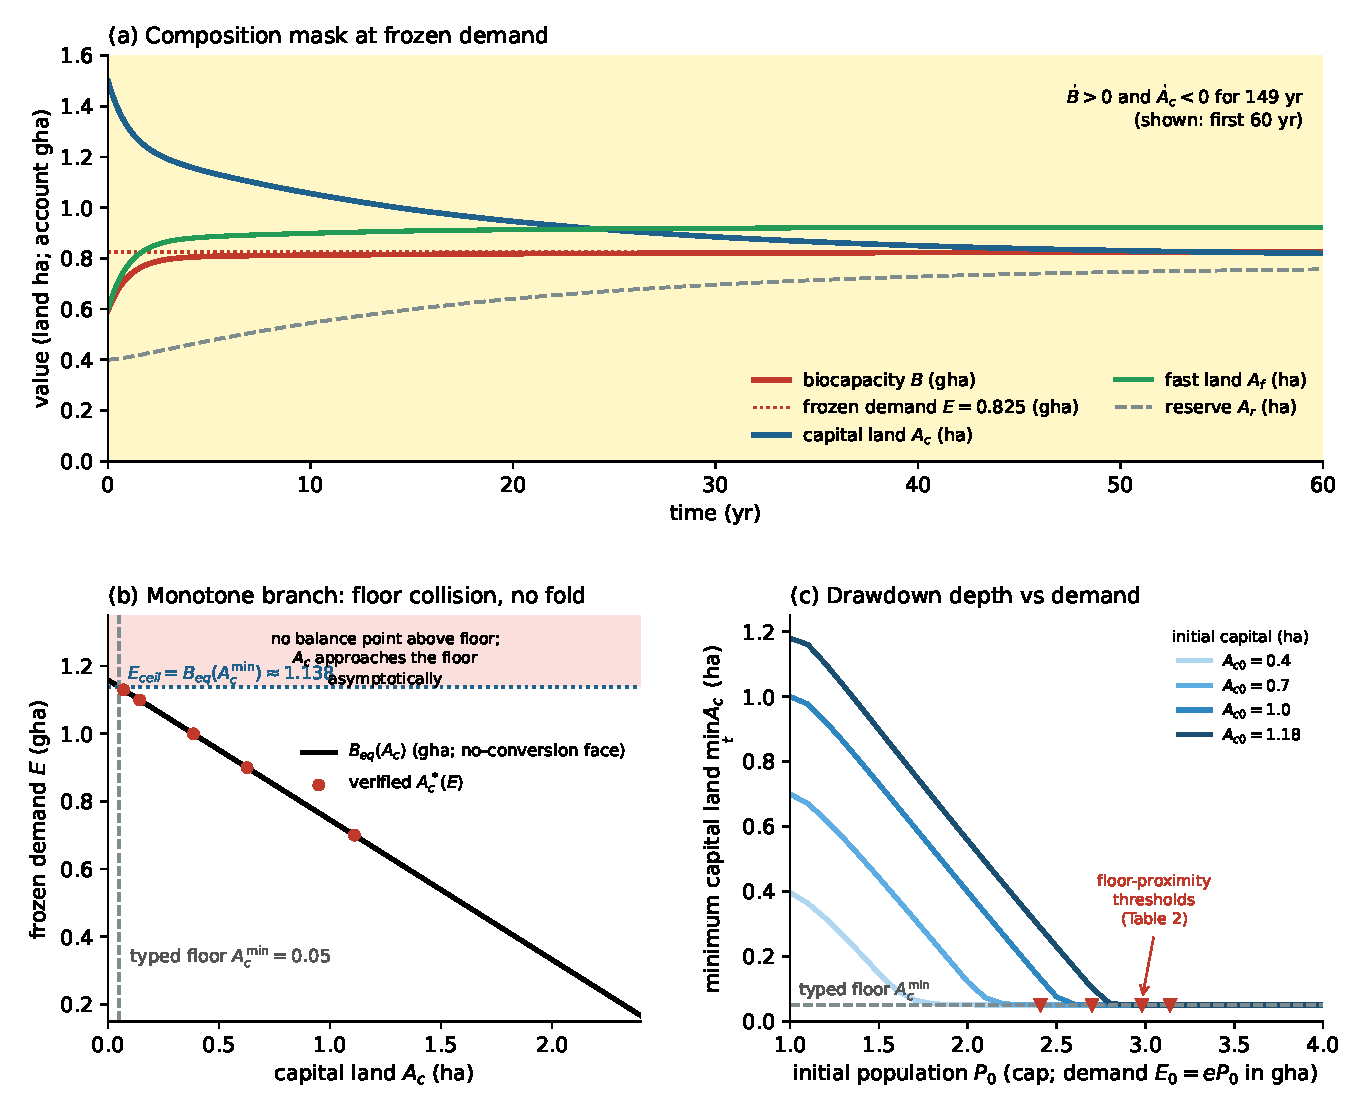
\includegraphics[width=\textwidth]{fig1_model_dynamics}
\caption{Baseline model results (Table~\ref{tab:params}). Account amounts $B$ and $E$ are in gha, land areas are in ha, and population is in cap. (a) Frozen demand ($E=0.825$\,gha), restoration off, and initial conditions $A_{f0}=0.6$\,ha, $A_{c0}=1.5$\,ha, and $q_0=0.9$. $B$ rises from $0.594$ to $0.825$\,gha as $A_c$ falls from $1.500$ to $0.808$\,ha and $A_f$ rises from $0.600$ to $0.923$\,ha. Shading marks the interval with $\dot B>0$ and $\dot A_c<0$ (about $149$\,yr; only the first $60$\,yr are shown). Within $25$\,yr, $98\%$ of the rise in $B$ and $85\%$ of the fall in $A_c$ occur. (b) Fixed-demand balance relation $B_{eq}(A_c)$; the listed balance areas are $A_c^*(E)=1.110$, $0.626$, $0.385$, $0.143$, and $0.070$\,ha at $E=0.70$, $0.90$, $1.00$, $1.10$, and $1.13$\,gha. The curve meets the minimum $A_c=0.05$\,ha at $\Eceil\approx1.138$\,gha; no balance point is admissible at higher demand. (c) Endogenous-demand runs with $\tau_g=20$\,yr, $\tau_p=25$\,yr, and $\chi_r=0.10$\,gha$^{-1}$\,yr$^{-1}$. For each initial area $A_{c0}$, the minimum area reached varies continuously and monotonically with $P_0$ ($E_0=eP_0$). The floor is approached asymptotically. Triangles mark the proximity values in Table~\ref{tab:model}, defined as within $10^{-6}$\,ha of the floor; no discontinuity is observed.}
\label{fig:model}
\end{figure}

\subsection{Fixed demand leads to a minimum-area boundary, not a fold}\label{sec:ceiling}

In endogenous-demand runs, population eventually reaches carrying capacity, demand matches the available account total, and the shortfall closes. Conversion then stops. We use a separate fixed-demand comparison to map where that balance point lies as demand changes. Its constraint $A_c\ge\Acmin$ is a \emph{typed floor}: it protects one land class, not the aggregate.

\begin{proposition}[Balance point, demand ceiling and affine deficit-side dynamics]\label{prop:ceiling}
For this reduced comparison, hold demand at $E$, switch off the technology boost and restoration, set debt $D=0$, and fix quality at $q=q_{\max}$. This quality is the attractor of \eqref{eq:q} for $q(0)>0$. Let $k=\mu/(\mu+\eta_f)$ and
\begin{equation}\label{eq:Beq}
B_{eq}(A_c)=b_{f0}\,k\,(A_{tot}-A_c)+b_cA_c=b_{f0}kA_{tot}-(b_{f0}k-b_c)A_c .
\end{equation}
\begin{enumerate}[label=(\roman*)]
\item With no conversion ($S=0$), reserve-to-fast maintenance balances fast-land retirement. This gives $A_f=k(A_{tot}-A_c)$ and $A_r=(1-k)(A_{tot}-A_c)$, where $k=\mu/(\mu+\eta_f)$. The resulting total is $B_{eq}(A_c)$. If $b_{f0}k>b_c$, this total decreases as $A_c$ increases, so there is at most one balance point $B_{eq}(A_c^*)=E$:
\begin{equation}\label{eq:Acstar}
A_c^*(E)=\frac{b_{f0}kA_{tot}-E}{b_{f0}k-b_c}.
\end{equation}
The algebraic solution is feasible when $B_{eq}(A_{tot})\le E\le\Eceil$, where $\Eceil=B_{eq}(\Acmin)$. It lies above the minimum area exactly when $E<\Eceil$. At lower demand, the algebraic root lies above $A_{tot}$, and every feasible no-conversion allocation already supplies at least $E$.
\item While shortfall is positive and conversion is not yet limited by the minimum-area constraint, the land subsystem is affine in $z=(A_f,A_c)$: $\dot z=Jz+c$, with
\begin{equation}\label{eq:J}
J=\begin{pmatrix}-\tconv^{-1}-\mu-\eta_f & -\mu-\dfrac{b_c}{b_f\tconv}\\[8pt] \tconv^{-1} & \dfrac{b_c}{b_f\tconv}\end{pmatrix},
\qquad \det J=\frac{\mu+\eta_f}{\tconv}\Big(k-\frac{b_c}{b_f}\Big),
\end{equation}
and $\operatorname{tr}J<0$. The matrix does not depend on demand or on the current state. Its determinant is positive exactly when $B_{eq}$ decreases, and its fixed point is the balance point in (i). For $B_{eq}(A_{tot})\le E<\Eceil$, trajectories that remain in this regime approach that point at rates set by the eigenvalues of $J$. For $E>\Eceil$, the balance point would lie below the allowed minimum: $A_c$ approaches $\Acmin$ asymptotically and the shortfall tends to $S^*=E-\Eceil>0$. Thus the reduced balance curve meets the minimum-area boundary; it does not turn back or form a fold. The leading eigenvalue does not approach zero at $E=\Eceil$, and the reduced equilibrium relation has no hysteresis. These conclusions hold under the stated assumptions and do not imply that the realized land allocation is independent of its history.
\item Above the demand ceiling, with degradation active, debt approaches a unique value $D^*(E)$ satisfying $\eta D=E-B_{eq}(\Acmin;D)$, where $B_{eq}(\cdot;D)$ uses yield $b_{f0}e^{-\alpha D}$. This result requires $\eta>\alpha b_{f0}k(A_{tot}-\Acmin)$; the equilibrium debt increases with demand.
\end{enumerate}
\end{proposition}

\begin{proof}
(i) With $S=0$ and $R_{rc}=0$, \eqref{eq:Af} gives $\mu A_r=\eta_fA_f$, hence $A_r/A_f=\eta_f/\mu$ and, with $A_r=A_{tot}-A_f-A_c$, $A_f=k(A_{tot}-A_c)$; substituting into \eqref{eq:B} with $q=q_{\max}$ ($\Ups=b_c$) and $D=0$ gives $B=B_{eq}(A_c)$, and $S=0$ requires $B\ge E$. Strict monotonicity and \eqref{eq:Acstar} follow from $b_{f0}k>b_c$. (ii) On the deficit side $u_c=(E-b_fA_f-b_cA_c)/(b_f\tconv)$ is affine in $z$; substituting into \eqref{eq:Ac}--\eqref{eq:Af} with $A_r=A_{tot}-A_f-A_c$ gives $J$ and a constant vector $c$ by direct differentiation; $\det J$ follows by expansion, and $\operatorname{tr}J=-\tconv^{-1}(1-b_c/b_f)-\mu-\eta_f<0$ for $b_c<b_f$. The fixed point solves $u_c=0$ and $\mu A_r=\eta_fA_f$, i.e.\ it is the balance point. Because $J$ is constant, convergence rates are constant along the branch. (iii) The map $D\mapsto\eta D+B_{eq}(\Acmin;D)-E$ is continuous, negative at $D=0$ when $E>\Eceil$, tends to $+\infty$, and is strictly increasing when $\eta>\alpha b_{f0}k(A_{tot}-\Acmin)\ge-\partial_DB_{eq}$; hence it has a unique root, which increases with $E$.
\end{proof}
The proposition describes the reduced equilibrium relation; it does not erase the history of the full model. With restoration off and no reverse conversion, $A_c$ stops falling when the shortfall closes but remains below its pre-overshoot level. Quality continues to evolve separately, so $\Ups(q)$ may still change. This is path dependence in the modeled allocation, not perpetual decline at equilibrium or a claim about real ecosystems.

At baseline, $k=0.5455$, the balance-branch slope parameter is $b_{f0}k-b_c=0.414$\,gha\,ha$^{-1}$, and the area floor is reached at $\Eceil=1.138$\,gha. Equation~\eqref{eq:Acstar} gives balance areas of $1.110$, $0.626$, $0.385$, $0.143$, and $0.070$\,ha at demands of $0.70$, $0.90$, $1.00$, $1.10$, and $1.13$\,gha; these match the integrated equilibria in Fig.~\ref{fig:model}b. The deficit-side eigenvalues are real and negative ($-0.0537$ and $-0.998$\,yr$^{-1}$). Across the tested fast-land yields, the leading eigenvalue shifts from $-0.0522$ to $-0.0556$\,yr$^{-1}$ without changing sign (Table~\ref{tab:model}a). The baseline composition premium $\dconv(q^*)=+0.784$\,gha\,ha$^{-1}$ follows from representative settings; it is not an empirically estimated yield difference between land classes.

Above the ceiling, debt approaches a finite fixed point when the stated repayment condition holds. At $E=1.158$ and $1.238$\,gha, the calculated equilibria are $D^*=1.19$ and $5.38$\,gha\,yr; numerical integration gives $1.21$ and $5.39$\,gha\,yr. The condition holds at baseline because $\alpha b_{f0}k(A_{tot}-\Acmin)=0.034$\,yr$^{-1}<\eta=0.05$\,yr$^{-1}$. Thus, under fixed demand, debt saturates rather than growing without bound.

Critical slowing down describes a fold approach in which the slow return rate tends to zero and the return time $T_{ret}\approx-1/\lambda_1$ grows. That signature is absent on this reduced branch: its linearization is constant, $\lambda_1$ remains negative, and return time stays near $19$\,yr as $E$ approaches $\Eceil$. The modeled warning is instead the approach of the typed state $A_c$ to its floor—information an aggregate-only observation cannot provide.

When population responds to supply, the minimum $A_c$ varies continuously and monotonically with initial population $P_0$ for each starting area $A_{c0}$ (Fig.~\ref{fig:model}c). Because $u_c\le(A_c-\Acmin)/\tconv$, the floor is approached asymptotically rather than crossed. A larger initial capital-land area supports a larger $P_0$ before the run approaches the floor.

Table~\ref{tab:model}b reports the initial populations at which $A_c$ comes within $10^{-2}$, $10^{-4}$, and $10^{-6}$\,ha of its minimum. These are tolerance-defined proximity values, not abrupt thresholds. At the tightest tolerance, the values are $2.41$, $2.70$, $2.98$, and $3.14$\,cap for $A_{c0}=0.40$, $0.70$, $1.00$, and $1.18$\,ha, respectively; they rise with starting area, with no jump at any tested tolerance.

At $A_{c0}=1.0$\,ha, the $10^{-6}$\,ha proximity value shifts by at most $0.001$\,cap across $\tau_g=5$, $20$, and $40$\,yr (SI Table S2). The comparison is limited to those settings. Switching surplus-gated restoration on leaves the tested threshold unchanged to three decimals because the gate is inactive while $B<E$ (SI~\S S4).

\begin{table}[!htbp]
\centering\small
\caption{Model results at the baseline parameter set. (a) At $q^*=q_{\max}/2$ ($\Ups(q^*)=0.066$\,gha\,ha$^{-1}$), the table reports $\dconv(q^*)$, the eigenvalues of the deficit-side matrix $J$ in \eqref{eq:J}, and the demand ceiling across a sweep of $b_f$; all other parameters are at baseline. (b) For endogenous-demand runs with $A_{f0}=0.6$\,ha, $q_0=0.9$, $\tau_g=20$\,yr, and $\tau_p=25$\,yr, the table reports the initial population $P_0$ at which the minimum $A_c$ comes within the stated distance of the floor $\Acmin=0.05$\,ha. The first two columns use a $P_0$ grid with step $0.1$ ($\Delta t=0.1$\,yr, $T=400$\,yr); the final column uses bisection with the $10^{-6}$\,ha proximity criterion ($\Delta t=0.05$\,yr, $T=1000$\,yr). Because drawdown depth varies continuously with $P_0$ (Fig.~\ref{fig:model}c), these values define proximity bands, not a single threshold.}
\label{tab:model}
\begin{tabular}{l l l l l}
\toprule
\multicolumn{5}{l}{(a) Fast-land yield sweep (all rows composition-premium, $\dconv>0$)}\\
$b_f$ (gha\,ha$^{-1}$) & $\dconv(q^*)$ (gha\,ha$^{-1}$) & $\lambda_1$ (yr$^{-1}$) & $\lambda_2$ (yr$^{-1}$) & $\Eceil$ (gha) \\
\midrule
$0.60$ & $+0.534$ & $-0.0522$ & $-0.975$ & $0.804$ \\
$0.85$ (baseline) & $+0.784$ & $-0.0537$ & $-0.998$ & $1.138$ \\
$1.20$ & $+1.134$ & $-0.0547$ & $-1.014$ & $1.606$ \\
$2.00$ & $+1.934$ & $-0.0556$ & $-1.029$ & $2.675$ \\
\bottomrule
\end{tabular}

\medskip
\begin{tabular}{l l l l}
\toprule
\multicolumn{4}{l}{(b) Initial population $P_0$ (cap) at which $\min_tA_c$ approaches $\Acmin$ to within:}\\ 
$A_{c0}$ (ha) & within $10^{-2}$\,ha & within $10^{-4}$\,ha & within $10^{-6}$\,ha \\
\midrule
$0.40$ & $\approx1.8$ & $\approx2.1$ & $\approx2.41$ \\
$0.70$ & $\approx2.2$ & $\approx2.4$ & $\approx2.70$ \\
$1.00$ & $\approx2.6$ & $\approx2.8$ & $\approx2.98$ \\
$1.18$ & $\approx2.8$ & $\approx3.0$ & $\approx3.14$ \\
\bottomrule
\end{tabular}
\end{table}

\subsection{Technology gains are finite; debt depends on the shortfall}\label{sec:bounded}

The technology boost and debt both change fast-land yield $b_f$, but in different ways. The boost has a fixed ceiling. Debt can accumulate while a shortfall persists, then approaches a finite level if that shortfall settles.

\begin{proposition}[The technology boost is capped; debt depends on the shortfall]\label{prop:bounded}
Under \eqref{eq:bf}--\eqref{eq:Tb}:
\begin{enumerate}[label=(\roman*)]
\item The technology factor $(b_{f0}+T_b(t))/b_{f0}$ stays between $1$ and $1+\Delta b/b_{f0}$. Its log-scale gain is therefore bounded by $\ln(1+\Delta b/b_{f0})$ for all time ($0.78$ at baseline).
\item Debt satisfies $D(t)\le\max\{D(0),\ \sup_{s\le t}\pos{E-B}(s)/\eta\}$. If the shortfall settles at $S^*$, then $D$ tends to $S^*/\eta$. The resulting reduction in fast-land yield depends on the size of that sustained shortfall.
\item The debt-related yield loss exceeds the largest possible technology gain once the sustained shortfall exceeds $S^\dagger=(\eta/\alpha)\ln(1+\Delta b/b_{f0})$, which is $1.30$\,gha at baseline.
\end{enumerate}
With additive degradation, $b_f=b_{f0}+T_b-\alpha D$, the two effects enter symmetrically; the comparison in (iii) then reduces to $\Delta b$ versus $\alpha D^*$. The asymmetry above follows from the model's multiplicative form.
\end{proposition}

\begin{proof}
(i) is $0\le T_b\le\Delta b$. (ii) From \eqref{eq:D}, $\dot D\le\bar S-\eta D$ with $\bar S=\sup_{s\le t}\pos{E-B}$, so $D(t)\le\max\{D(0),\bar S/\eta\}$ by comparison; if $\pos{E-B}\to S^*$ then $D\to S^*/\eta$. (iii) compares $\alpha S^*/\eta$ with $\ln(1+\Delta b/b_{f0})$.
\end{proof}

For a fixed persistent shortfall, debt approaches $S^*/\eta$; the larger the shortfall, the higher the limiting debt and the lower the fast-land yield. At baseline, the crossover $S^\dagger\approx1.30$\,gha exceeds $B$. The typed area constraint binds before debt erosion can exceed the maximum technology gain, although debt still reduces $b_f$ over time.

The matched technology-wave experiment shows why the debt response depends on the observation window and starting population. At $P_0=1.0$\,cap, peak debt over $0$--$250$\,yr is $0.02020$\,gha\,yr with the wave and $0.00813$\,gha\,yr without it (ratio $2.49$). At $P_0=1.2$\,cap, the all-time maximum is lower with the wave ($0.05104$ versus $0.06122$\,gha\,yr), but the post-midpoint maximum is higher ($0.02518$ versus $0.01085$\,gha\,yr; ratio $2.32$). The post-midpoint window includes the logistic wave's continued rise. These are conditional model comparisons, not forecasts or empirical estimates (SI~\S S8).

\subsection{Recovery requires an explicit, gated restoration flow}\label{sec:recovery}

Conversion moves area from capital land to fast use. In the baseline, there is no reverse route: fast-land retirement returns area to reserve, not to $A_c$. A lower population or a closed shortfall therefore does not, by itself, restore capital-land area. If $\chi_r=0$, $A_c$ remains at its post-conversion value.

For $A_{c0}=1.0$\,ha and $P_0=2.0$\,cap, the endogenous-demand run reaches $A_c=0.398$\,ha within four years and stays there without restoration. With surplus-gated restoration ($\chi_r=0.10$\,gha$^{-1}$\,yr$^{-1}$), it recovers to $0.828$\,ha, or $\mathcal R_c=0.71$ (SI~\S S4.3).

The gate determines when restoration can act. A surplus-gated flow is off during shortfall and may continue after surplus returns while population adjusts; a target cap is needed to stop at a specified endpoint (SI~\S S4.4). A deficit-gated flow acts during shortfall, when supply is already insufficient. At the tested rates, conversion is stronger and drawdown continues. These are conditional comparisons; neither gate is universally preferable.

\subsection{NFA account composition, 1961--2023}

\label{sec:empirical}

We use complete world observations from NFA Edition 2026 through 2023 and exclude the estimated 2024--2025 rows. The 1961--2022 sensitivity holds the account edition and population series fixed.

From 1961 to 2023, total biocapacity account value $B$ rises from $9.7254\times10^9$ to $12.1428\times10^9$\,gha ($+24.86\%$; $\Delta\ln B=+0.221997$). Population rises from $3.06487$ to $8.09173$ billion. Over the same period, $B/P$ falls from $3.17319$ to $1.50065$\,gha\,person$^{-1}$ ($-52.71\%$; $\Delta\ln(B/P)=-0.748840$), while production footprint per person rises from $2.19700$ to $2.56462$\,gha\,person$^{-1}$ ($+16.73\%$). The ratio $E_{\mathrm{prod}}/B$ increases from $0.69236$ to $1.70901$ and first exceeds one in 1973.

The exact identity $\Delta\ln B=\Delta\ln P+\Delta\ln(B/P)$ gives $+0.970837-0.748840=+0.221997$. It separates population scale from biocapacity per person; it does not explain why either changed. In the same-edition 1961--2022 sensitivity, $\Delta\ln B=+0.219497$, $B/P$ falls $52.41\%$, production footprint per person rises $17.70\%$, and 1973 remains the first year with $E_{\mathrm{prod}}/B>1$ (SI~\S S5).

The component accounts explain the aggregate movement (Fig.~\ref{fig:composition}; Table~\ref{tab:nfa_components}). Cropland contributes $+24.06$ percentage points to the total $+24.86\%$ change (about $96.8\%$ of the net change). Forest biocapacity contributes $-5.95$ points, grazing land $-0.27$, fishing grounds $-0.42$, and built-up land $+7.44$. The non-cropland account sum, including built-up land, changes by only $+0.80$ points ($1.0092\times$) as these account movements offset one another.

The components sum to the total within workbook rounding at both endpoints. These figures describe account composition: they do not measure forest biomass, soil condition, wetland extent, fish biomass, or model area $A_c$. Built-up land is an NFA accounting class, not ecological capital.

\begin{samepage}
An external cropland-area series and cereal-yield index provide a separate, illustrative account split (SI~\S S5). Anchored to the measured 1961 NFA cropland share ($\phi_0=0.128647$, about $12.86\%$), the exact log-change decomposition assigns $+0.268662$ to the cereal-yield index, $+0.037710$ to area, and $-0.084375$ to the residual; the three terms sum to $\Delta\ln B=+0.221997$. This identity is exact for the stated proxy, but the allocation changes with the anchor and is not a physical-stock attribution.\par
\end{samepage}

\begin{figure}[!htbp]
\centering
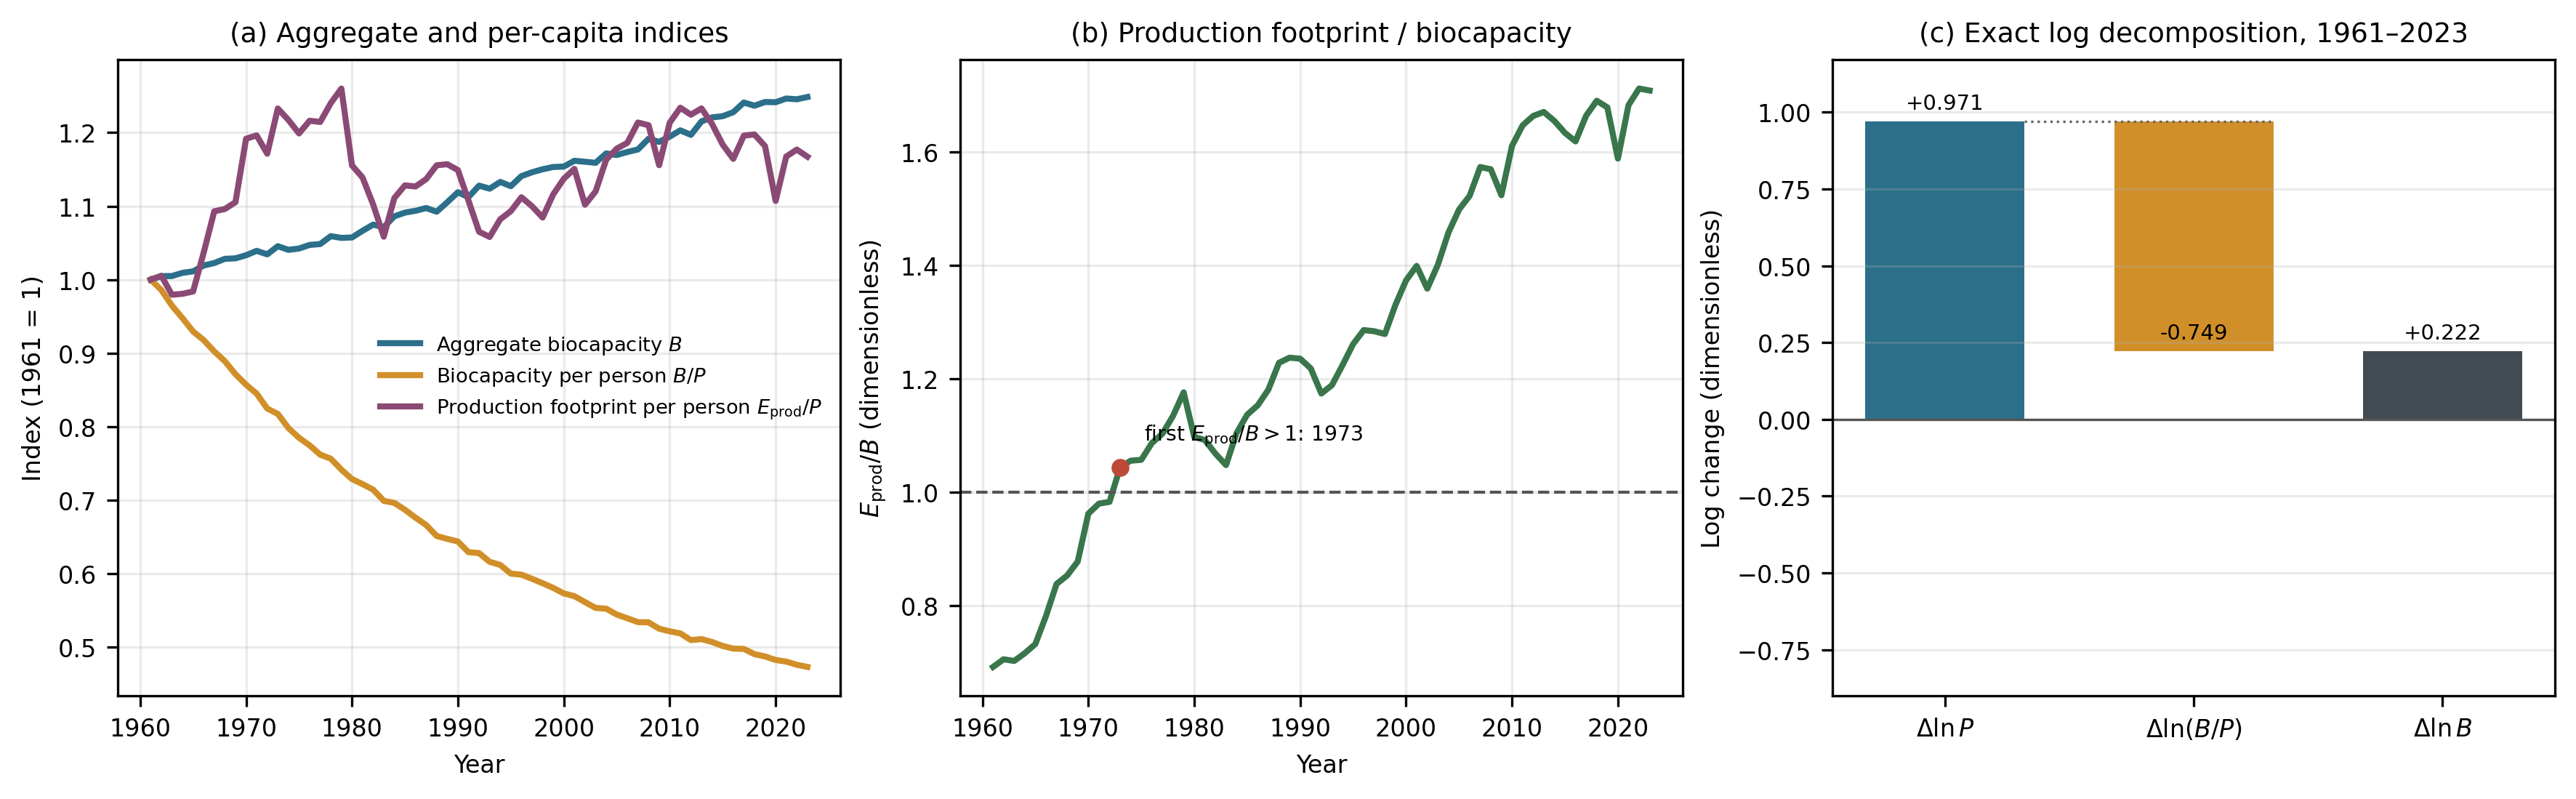
\includegraphics[width=\textwidth]{fig2_nfa_aggregation_face}
\caption{Aggregate and per-capita movements in NFA Edition 2026 (world, 1961--2023; complete observations). $B$ is total biocapacity, $E_{\mathrm{prod}}$ is the workbook's Global Ecological Footprint of Production, and $P$ is the single UN PopStat population series; per-capita values are calculated from totals. (a) Indices (1961 $=1$) of $B$, $B/P$, and $E_{\mathrm{prod}}/P$. (b) $E_{\mathrm{prod}}/B$, first above one in 1973. (c) Exact log identity $\Delta\ln B=\Delta\ln P+\Delta\ln(B/P)$. Account values are in gha; plotted indices, ratios, and log changes are dimensionless. The 2024--2025 estimated rows are excluded.}
\label{fig:aggregation}
\end{figure}

\begin{table}[!htbp]
\centering\footnotesize
\caption{NFA Edition 2026 biocapacity-account endpoint ratios and contributions. Contributions are $100\,[B_i(T)-B_i(1961)]/B(1961)$ percentage points; endpoint ratios are $B_i(T)/B_i(1961)$. The 2022 sensitivity is from the same edition. All entries are account values, not physical-stock measurements.}
\label{tab:nfa_components}
\begin{tabularx}{\textwidth}{@{}Xrrrr@{}}
\toprule
Component & \shortstack{2023\\ratio} & \shortstack{2023 contribution\\(pp of $B_{1961}$)} & \shortstack{2022 sensitivity\\ratio} & \shortstack{2022 contribution\\(pp of $B_{1961}$)} \\
\midrule
Cropland & 2.8701 & $+24.0577$ & 2.8514 & $+23.8183$ \\
Grazing land & 0.9828 & $-0.2688$ & 0.9815 & $-0.2890$ \\
Forest biocapacity & 0.8996 & $-5.9525$ & 0.9019 & $-5.8137$ \\
Fishing grounds & 0.9627 & $-0.4212$ & 0.9596 & $-0.4559$ \\
Built-up land$^{\dagger}$ & 8.7935 & $+7.4416$ & 8.6298 & $+7.2854$ \\
Non-cropland sum$^{\dagger}$ & 1.0092 & $+0.7990$ & 1.0083 & $+0.7267$ \\
\midrule
Total biocapacity & 1.2486 & $+24.8568$ & 1.2454 & $+24.5450$ \\
\bottomrule
\end{tabularx}
\begin{flushleft}\footnotesize
$^{\dagger}$Built-up land is not ecological capital; the non-cropland account sum includes it. Component sums match total biocapacity within workbook rounding. \end{flushleft}
\end{table}

\begin{figure}[!htbp]
\centering
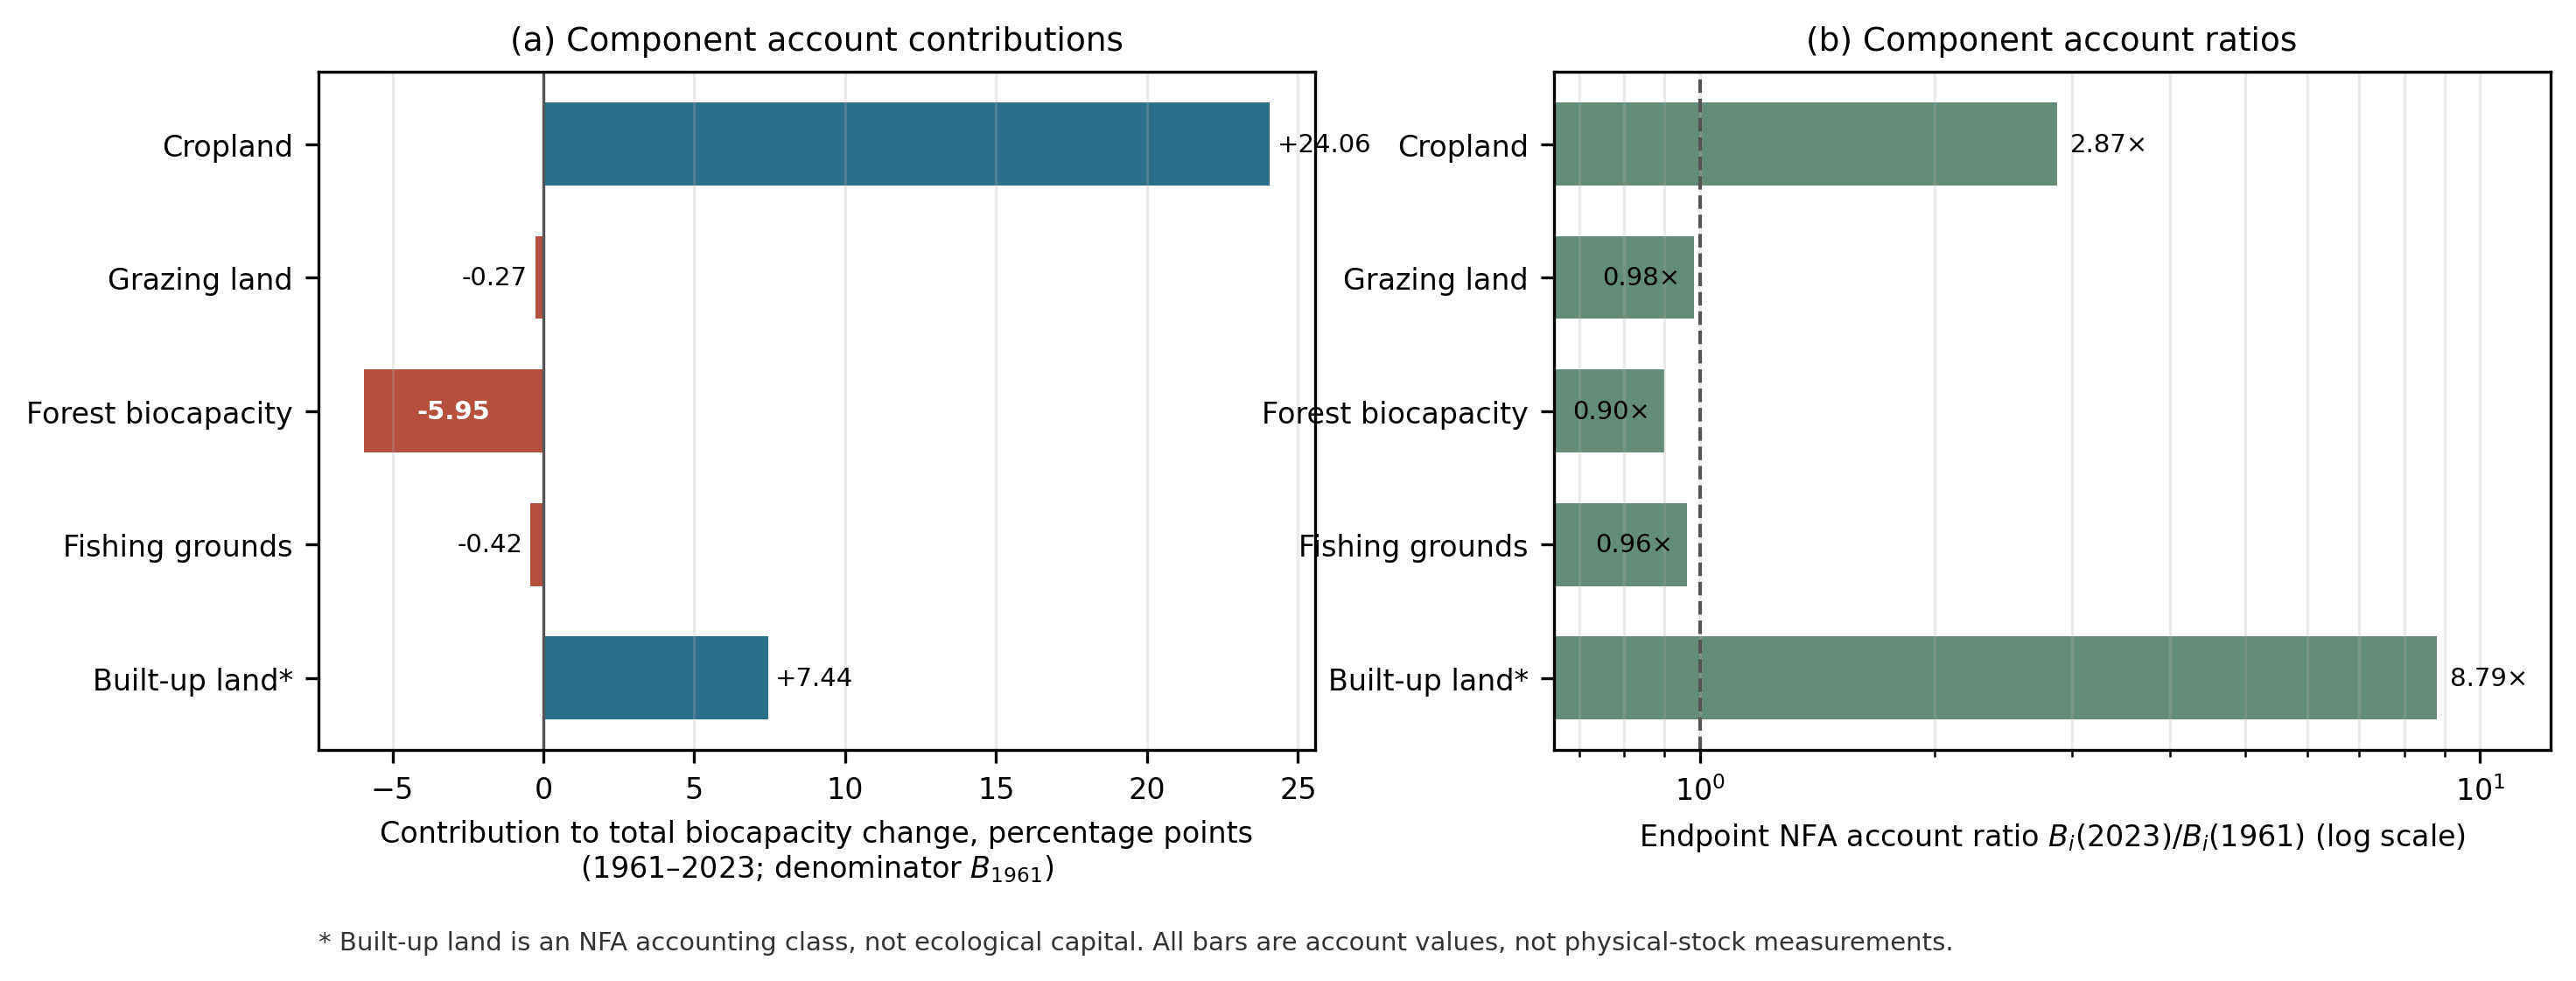
\includegraphics[width=0.95\textwidth]{fig3_composition_attribution}
\caption{NFA Edition 2026 land-type biocapacity-account changes, world, 1961--2023. (a) Component contributions in percentage points of $B_{1961}$. (b) Endpoint ratios $B_i(2023)/B_i(1961)$. “Forest biocapacity” is the workbook's exact label. All bars are account values, not measurements of physical stocks; built-up land is an NFA accounting class, not ecological capital.}
\label{fig:composition}
\end{figure}

\subsection{Falsifiable predictions}\label{sec:predictions}

The model gives five testable implications. A field test of the composition mechanism needs component information: capital-land area, fast-land area, and relevant land-cover or yield observations.
\begin{enumerate}[label=P\arabic*.,leftmargin=2.2em]
\item \textbf{A composition mask requires a positive conversion contribution.} In the baseline frozen-demand run, $B$ rises while $A_c$ falls for a finite interval (Fig.~\ref{fig:model}a). The conversion term is positive when $\dconv>0$; whether total $B$ rises also depends on all other active terms. With full availability, conversion begins only when $E/B>1$. Reserved-share results are a separate extension and can allow conversion when $E/B\le1$.
\item \textbf{The duration is set by model rates and the initial shortfall.} The slow return rate $\lambda_1$, together with $\tconv$, $\mu$, $\eta_f$, and $b_c/b_f$, sets the timescale; $\dconv$ and the starting shortfall affect the size of the adjustment. In the baseline, most conversion occurs within one to two e-folding times.
\item \textbf{The reduced balance branch has no fold-related warning.} Return time stays finite as demand approaches the ceiling, and the modeled $A_c$ approaches a typed floor. This is a result for the reduced comparison, not a general stability claim for the delayed system.
\item \textbf{Floor proximity depends on starting area.} The initial population at which a run approaches the floor rises with $A_{c0}$ (Table~\ref{tab:model}b). At $A_{c0}=1.0$\,ha, the $10^{-6}$\,ha proximity value changes by at most $0.001$\,cap over $\tau_g=5,20,40$\,yr (SI Table S2); this does not establish insensitivity outside the tested range.
\item \textbf{Recovery requires an explicit return flow.} Lower demand alone does not restore $A_c$. Surplus-gated restoration is inactive during shortfall; deficit-gated restoration acts then and can further reduce provision.
\end{enumerate}
Aggregate $B$ alone cannot test these implications. Testing the composition mechanism requires independent observations or defensible proxies for $A_c$ and fast-land yield $b_f$; testing delay, recovery, and demand-threshold responses also requires relevant time series and demographic or intervention data.

\clearpage
\section{Discussion}\label{sec:discussion}

\subsection{What the two-land model shows}

The model isolates a simple compositional mechanism; it does not reconstruct a real landscape. When fast land contributes more per hectare than capital land, conversion raises $B$ at the margin even while $A_c$ falls. The net change in $B$ can still have the opposite sign because maintenance, retirement, and quality change act at the same time. The technology term is capped, while debt responds to the size and persistence of the shortfall (Propositions~\ref{prop:mask} and~\ref{prop:bounded}) \citep{Schaefer1954,May1973,Meadows1972,Meadows2004,WackernagelRees1996,BranderTaylor1998}.

The fixed-demand comparison answers a narrower question. Under its stated assumptions, the balance relation has one branch and meets the area floor without folding back. That rules out a fold, hysteresis, or critical slowing on this reduced branch; it does not establish stability for every trajectory of the delayed system. In the full model, the path still matters: without a return flow, $A_c$ remains below its pre-overshoot level after conversion stops, although it no longer declines at the balance point. Recovery depends on the timing and gate of the explicit restoration flow.

SI~\S S7 presents a separate one-stock comparator, not a reduction of the two-land model. Its state $A$ uses comparator-specific units and is not $A_c$. With the illustrated constant parameters and no debt, its equilibrium relation is $B(A)=(b+b_G\rho)A-(b_G\rho/A_{\max})A^2$, with $P=B(A)/e$. At those settings, $b_G\rho<b$, so the relation is monotone; other parameter choices would be needed for an interior maximum. Its neutral equilibrium family and selected delay paths apply only to that formulation. They do not establish a fold, a general critical delay, or a collapse mechanism in the two-land model.

Early-warning indicators such as rising autocorrelation and variance are associated with approaching a fold \citep{Scheffer2001}. This reduced branch reaches a typed area boundary instead. Those fold-related indicators therefore need not rise first; their absence is not evidence that the system is safe. In the model, the relevant state to follow is $A_c$, which the aggregate alone cannot reveal.

\begin{table}[!htbp]
\centering\footnotesize
\caption{Equilibrium, trajectory, and tested delay-sensitivity properties under the stated assumptions.}
\label{tab:neg}
\begin{tabularx}{\textwidth}{>{\raggedright\arraybackslash}p{0.34\textwidth} l >{\raggedright\arraybackslash}X}
\toprule
Property & Finding & Scope \\
\midrule
Fold on the reduced frozen-demand branch & Absent & $B_{eq}(A_c)$ is strictly monotone; the balance point collides with the typed floor at $\Eceil\approx1.138\,\mathrm{gha}$ (Proposition~\ref{prop:ceiling}) \\
Critical slowing as $E\to\Eceil$ & Absent & The slow eigenvalue remains negative and constant along the reduced branch \\
Hysteresis of the frozen-demand equilibrium relation & Absent & There is at most one feasible balance point; this does not imply history independence of realized states \\
Path dependence of realized $A_c$ & Present, conditional & With $R_{rc}=0$, one-way conversion leaves $A_c$ below its pre-overshoot level after shortfall closure, while $\dot A_c=0$ at equilibrium \\
Discontinuous response to endogenous demand & Not observed & In the reported runs, minimum $A_c$ varies continuously and monotonically with initial population; proximity thresholds depend on tolerance \\
Regeneration-delay sensitivity ($\tau_g$, with $\tau_p=25$\,yr) & Small in tested range & At $A_{c0}=1.0$\,ha, the delayed-quality $10^{-6}$\,ha threshold varies by $0.001$\,cap across $\tau_g=5,20,40$\,yr (SI Table S2); this does not establish invariance outside that range \\
\bottomrule
\end{tabularx}
\end{table}
\clearpage

\subsection{Measurement implications}

A biocapacity total is a value-weighted account, not a census of land classes. Even with fixed per-hectare values, the total and the area-conservation rule leave multiple feasible land allocations (Proposition~\ref{prop:mask}(iii)). Independent measures of land area and productivity are needed to distinguish those allocations. Related transition-assessment work studies the same general issue of compensation under component floors, but in a separate finite-plan setting \citep[Sections~2 and 4 of][]{Abaee2026b}. There, the compensatory protocol accepts states even when no available plan meets every component floor (Theorem~2 in \citet{Abaee2026b}). Theorem~4(iii) in \citet{Abaee2026b} identifies an exact interval of diagonal-gap states on its witness-defined region that each positive elasticity falsely certifies as safe; no positive-elasticity member is uniformly safe on that region. This is a scoped result about the companion's region, not a general claim about all transition systems. A typed floor can also be violated during a transition even if an endpoint later recovers.

The NFA results describe account composition. Total biocapacity account value rose while biocapacity per person fell; cropland's account contribution offset declines in other categories, and built-up land is an accounting class rather than ecological capital. None of these movements measures forest biomass, soil condition, wetland extent, fish biomass, or $A_c$. In particular, a decline in Forest biocapacity is not a measurement of declining forest biomass. The account quantities use gha, with the annual basis implicit; per-person values use gha per person. The endpoint and same-edition sensitivity results are reported in Section~\ref{sec:empirical} and SI~\S S5 \citep{Lo2026NFA,Borucke2013,Blomqvist2013,GiampietroSaltelli2014,Galli2016,vdBerghGrazi2015}.

The crop-area/cereal-yield proxy is a separate account construction, not a measurement of the model's land classes. Its residual $C=B-\hat b_fA_f$ absorbs boundary and calibration differences; it is neither physical capital nor $\Ups(q)A_c$. The study did not assemble a common-boundary global physical-stock series, so it reports no physical-stock composite or global decline finding. The SI scoreboard specifies candidate measures and comparison requirements but contains no endpoint inventory. Any physical-stock comparison would need independent observations, consistent boundaries and units, and an explicit treatment of uncertainty, overlap, valuation, and substitution. SEEA Ecosystem Accounting likewise distinguishes extent and condition from ecosystem services and monetary presentations \citep{UN2021SEEA_EA}.

\subsection{Policy controls and limits}

The model compares three controls, not policy outcomes. A stop tied to $A_c=\Acmin$ preserves the modeled capital-land floor. A ceiling on $A_f$ or a governor that monitors only total $B$ does not guarantee that floor, because $B$ does not identify $A_c$.

The restoration gates also differ in timing. Surplus-gated restoration is inactive during a shortfall; deficit-gated restoration acts during the shortfall and can reduce provision further. This distinction parallels protective and mobilizing institutional feedback in related work \citep{Abaee2026a}. A shared reserved fraction makes conversion inactive while $E\le\sigma B$; with separate shares, the condition is $E\le\sigma_fY_f+\sigma_cY_c$. This reservation concerns annual human-available flow, not spatially protected area. Half-Earth is a spatial conservation target; the model neither maps protected areas nor evaluates that proposal \citep{Wilson2016}. Robustness to disturbances and parameter uncertainty remains untested.

\subsection{Relation to prior work}

The ledger companion distinguishes weak and strong sustainability as operating regimes according to whether material loops close at throughput. In its terms, a positive weighted sum ranks outcomes under weak sustainability, whereas componentwise adequacy is the strong-sustainability predicate \citep[Sections~1.1 and 10.1]{Abaee2026c}\footnote{The v50 PDF is present at the pinned commit. The checksum manifest lists the v49 article files but omits v50; the README dated 2026-09-19 does not explicitly label v49 or v50; and the v50 TeX header points to the v48 Markdown source.}. ECOMOD's $B$ is an annual biocapacity-account total. The link is an analogy about compensation, not an identity with the companion's material-flow ledger or a complete sustainability classification. The assessment companion studies aggregate measures and typed transition criteria in a separate finite-plan setting \citep{Abaee2026b}; the governance companion studies institutional feedback \citep{Abaee2026a}. The delays here represent ecological regeneration and demographic response, not institutional review.

\subsection{Limitations}

The model compresses forests, soils, wetlands, and other assets into one capital-land class with one quality state. Its regeneration rule, composition diagnostic, and demand ceiling are effective model quantities, not estimates for any one ecosystem. Most parameters are representative rather than fitted, and the model does not identify $b_c$, $b_{G,c}$, and $\rho_c$ separately. Recovery records give timescale context; they do not estimate the ecological delay $\tau_g$. We hold the per-person footprint constant, and the zero-repayment limit $\eta\to0$ is not analyzed.

The composition result depends on demand and the mechanisms included. The exact shortfall switch makes stability at $S=0$ one-sided, and reported floor thresholds depend on numerical tolerance and time step. NFA accounts combine area and yield, so they cannot identify those components separately. Replacing delayed regeneration $G_c(q(t-\tau_g))$ with current-quality regeneration $G_c(q(t))$ lengthens the demonstration mask by $1.3$\,yr and shifts the initial-population threshold by at most $0.001$\,cap in the tested comparison (SI~\S S3).

\section{Conclusions}\label{sec:conclusions}

A rising biocapacity total does not, by itself, tell us how its land classes changed. In the model, conversion raises $B$ at the margin when fast-land yield exceeds capital land's effective per-hectare value, even while $A_c$ falls. Whether the total rises overall also depends on other flows. In the representative run, $A_c$ falls $46.16\%$ and its modeled contribution falls $51.72\%$, while total model $B$ rises $39\%$. These are conditional model results, not measurements of global physical stocks.

The fixed-demand comparison follows one balance branch to the area floor without a fold, hysteresis, or critical slowing. That conclusion is limited to the reduced comparison. In the delayed model, the realized path depends on prior conversion; without restoration, the lower $A_c$ persists after the shortfall closes.

NFA Edition 2026 shows a different kind of evidence: account values. From 1961 to 2023, total biocapacity account value rises $24.86\%$, while $B/P$ falls $52.71\%$ and production footprint per person rises $16.73\%$. Cropland contributes $+24.06$ percentage points, Forest biocapacity $-5.95$, and built-up land $+7.44$ as an accounting class. These figures describe account composition, not physical stocks; they do not establish a global decline in biomass, soil, wetlands, fish, or model area $A_c$. The crop proxy is also an account construction, not a physical-stock measure.

The practical point is about information: component accounts help readers interpret an aggregate. The orchard is an analogy, not evidence of a measured global stock decline. One record tracks the annual harvest; another would require independent, comparable observations of the assets that support future harvests. A harvest total is not a census of the orchard.

\section*{Acknowledgments}

The author thanks Global Footprint Network for making its data publicly available; Mathis Wackernagel for his thoughtful review; the editors of \emph{Ecological Modelling} for their trust and support; and Arena.ai for its ingenuity and online tools.

\section*{Declarations}

\paragraph{Data availability} All empirical inputs are publicly available from the sources cited in the manuscript. Derived analysis data and model code will be deposited in a public GitHub repository and archived in Zenodo; repository and record details will be added after the deposit is complete.

\paragraph{Funding} No funding was received.

\paragraph{Competing interests} The author declares no competing interests.

\paragraph{CRediT authorship contribution statement} \textbf{Amin Abaee:} Conceptualization; Methodology; Software; Formal analysis; Writing -- original draft; Writing -- review \& editing.

\paragraph{Declaration of generative AI in scientific writing} DeepSeek AI and Claude (Anthropic) assisted with computational-reproducibility checks under the author's supervision; the author reviewed and edited the content and takes full responsibility for the publication.
\begin{thebibliography}{99}
\bibitem[{Abaee(2026a)}]{Abaee2026a} Abaee, A. (2026a). \emph{Governance delay and the stability of harvested stocks: mobilising and protective feedback rules, and the review interval as a design parameter}. Working paper (v41). \url{https://github.com/MIKEAA2020/general-sustainability/blob/2efaa62083f2007dec3446c15c475af88f0925f3/arena%20agent%201/paper%20rewrites/latex/paper4_delay_dynamics_v41.pdf}.
\bibitem[{Abaee(2026b)}]{Abaee2026b} Abaee, A. (2026b). \emph{Aggregation is a claim, not a presentation: the geometry of the acceptance gap between compensatory and noncompensatory transition assessment}. Working paper (v71). \url{https://github.com/MIKEAA2020/general-sustainability/blob/2efaa62083f2007dec3446c15c475af88f0925f3/arena%20agent%201/paper%20rewrites/latex/paper06_assessment_separation_v71.pdf}.
\bibitem[{Abaee(2026c)}]{Abaee2026c} Abaee, A. (2026c). \emph{Typed Flux Ledgers and Depletion Arithmetic: Conservation, Componentwise Diagnostics, and the Semantics of Depletion Horizons}. Working paper. PDF pinned to GitHub commit \url{https://github.com/MIKEAA2020/general-sustainability/blob/2efaa62083f2007dec3446c15c475af88f0925f3/paper3/latest-2026-09-19/manuscript/paper3_material_ledgers_v50.pdf}.
\bibitem[{Anderies(2000)}]{Anderies2000} Anderies, J. M. (2000). On modeling human behavior and institutions in simple ecological economic systems. \emph{Ecological Economics}, 35(3), 393--412.
\bibitem[{Becker et al.(2017)}]{Becker2017} Becker, W., Saisana, M., Paruolo, P. \& Vandecasteele, I. (2017). Weights and importance in composite indicators: Closing the gap. \emph{Ecological Indicators}, 80, 12--22.
\bibitem[{Blomqvist et al.(2013)}]{Blomqvist2013} Blomqvist, L., Brook, B. W., Ellis, E. C., Kareiva, P. M., Nordhaus, T. \& Shellenberger, M. (2013). Does the shoe fit? Real versus imagined ecological footprints. \emph{PLoS Biology}, 11(11), e1001700.
\bibitem[{Borucke et al.(2013)}]{Borucke2013} Borucke, M., Moore, D., Cranston, G., Gracey, K., Iha, K., Larson, J., Lazarus, E., Morales, J. C., Wackernagel, M. \& Galli, A. (2013). Accounting for demand and supply of the biosphere's regenerative capacity: The National Footprint Accounts' underlying methodology and framework. \emph{Ecological Indicators}, 24, 518--533.
\bibitem[{Brander and Taylor(1998)}]{BranderTaylor1998} Brander, J. A. \& Taylor, M. S. (1998). The simple economics of Easter Island: A Ricardo--Malthus model of renewable resource use. \emph{American Economic Review}, 88(1), 119--138.
\bibitem[{Calvin and Bond-Lamberty(2018)}]{CalvinBondLamberty2018} Calvin, K. \& Bond-Lamberty, B. (2018). Integrated human--Earth system modeling --- state of the science and future directions. \emph{Environmental Research Letters}, 13(6), 063006.
\bibitem[{Cohen(1995)}]{Cohen1995} Cohen, J. E. (1995). Population growth and Earth's human carrying capacity. \emph{Science}, 269(5222), 341--346.
\bibitem[{Dasgupta(2021)}]{Dasgupta2021} Dasgupta, P. (2021). \emph{The Economics of Biodiversity: The Dasgupta Review.} London: HM Treasury.
\bibitem[{Donges et al.(2017)}]{Donges2017} Donges, J. F., Winkelmann, R., Cornell, S. E., Lucht, W., Dyke, J. G., Rockstr\"om, J., Heitzig, J. \& Schellnhuber, H. J. (2017). Closing the loop: Reconnecting human dynamics to Earth system science. \emph{The Anthropocene Review}, 4(2), 151--157.
\bibitem[{Erb et al.(2017)}]{Erb2017} Erb, K.-H., Luyssaert, S., Meyfroidt, P., Pongratz, J., Don, A., Kloster, S., Kuemmerle, T., Fetzel, T., Fuchs, R., Hasegawa, T., Haberl, H., et al. (2017). Land management: data availability and process understanding for global change studies. \emph{Global Change Biology}, 23(2), 512--533.
\bibitem[{Fischer et al.(2022)}]{Fischer2022} Fischer, S. M., Joy, M. K., Abrahamse, W., Milfont, T. L. \& Petherick, L. M. (2022). The use and misuse of composite environmental indices. \emph{bioRxiv}, 2022.03.15.484501. \url{https://doi.org/10.1101/2022.03.15.484501}.
\bibitem[{Global Footprint Network(2009)}]{GFNStandards2009} Global Footprint Network (2009). \emph{Ecological Footprint Standards 2009}. Global Footprint Network. \url{https://www.footprintnetwork.org/content/uploads/2019/05/Ecological_Footprint_Standards_2009.pdf}.
\bibitem[{Global Footprint Network(2019)}]{GFNGuidebook2019} Global Footprint Network (2019). \emph{Working Guidebook to the National Footprint Accounts 2019}. Global Footprint Network. \url{https://www.footprintnetwork.org/content/uploads/2019/05/National_Footprint_Accounts_Guidebook_2019.pdf}.
\bibitem[{Galli et al.(2016)}]{Galli2016} Galli, A., Giampietro, M., Goldfinger, S., Lazarus, E., Lin, D., Saltelli, A., Wackernagel, M. \& M\"uller, F. (2016). Questioning the ecological footprint. \emph{Ecological Indicators}, 69, 224--232.
\bibitem[{Giampietro and Saltelli(2014)}]{GiampietroSaltelli2014} Giampietro, M. \& Saltelli, A. (2014). Footprints to nowhere. \emph{Ecological Indicators}, 46, 610--621.
\bibitem[{Haberl et al.(2007)}]{Haberl2007} Haberl, H., Erb, K.-H., Krausmann, F., Gaube, V., Bondeau, A., Plutzar, C., Gingrich, S., Lucht, W. \& Fischer-Kowalski, M. (2007). Quantifying and mapping the human appropriation of net primary production in earth's terrestrial ecosystems. \emph{PNAS}, 104(31), 12942--12947.
\bibitem[{Henderson and Loreau(2018)}]{HendersonLoreau2018} Henderson, K. \& Loreau, M. (2018). How ecological feedbacks between human population and land cover influence sustainability. \emph{PLoS Computational Biology}, 14(8), e1006389.
\bibitem[{Hutchings and Reynolds(2004)}]{HutchingsReynolds2004} Hutchings, J. A. \& Reynolds, J. D. (2004). Marine fish population collapses: consequences for recovery and extinction risk. \emph{BioScience}, 54(4), 297--309.
\bibitem[{Hutchinson(1948)}]{Hutchinson1948} Hutchinson, G. E. (1948). Circular causal systems in ecology. \emph{Annals of the New York Academy of Sciences}, 50(4), 221--246.
\bibitem[{Krausmann et al.(2013)}]{Krausmann2013} Krausmann, F., Erb, K.-H., Gingrich, S., Haberl, H., Bondeau, A., Gaube, V., Lauk, C., Plutzar, C. \& Searchinger, T. D. (2013). Global human appropriation of net primary production doubled in the 20th century. \emph{PNAS}, 110(25), 10324--10329.
\bibitem[{Lo et al.(2026)}]{Lo2026NFA} Lo, K., Basnet, N., Miller, E., Srikanthalingam, B., Foley, B., Van Berkum, J. L., Long, A. H., Toneva, P., Ermina, M. \& Klinkenberg, C. (2026). \emph{National Ecological Footprint and Biocapacity Accounts, Edition 2026 (1961--2025): Results and metadata, version 1.0.} Prepared for Footprint Data Foundation by researchers at York University and the University of Iceland. Workbook: \url{https://footprint.info.yorku.ca/files/2026/04/NEFBA_Data_global_national_ecological_footprint_biocapacity.xlsx}; release notes: \url{https://footprint.info.yorku.ca/files/2026/04/NEFBA_ReleaseNotes.pdf}; data page: \url{https://footprint.info.yorku.ca/data/}.
\bibitem[{May(1973)}]{May1973} May, R. M. (1973). \emph{Stability and Complexity in Model Ecosystems.} Princeton: Princeton University Press.
\bibitem[{Meadows et al.(1972)}]{Meadows1972} Meadows, D. H., Meadows, D. L., Randers, J. \& Behrens, W. W. (1972). \emph{The Limits to Growth.} New York: Universe Books.
\bibitem[{Meadows et al.(1974)}]{Meadows1974} Meadows, D. L., Behrens, W. W., Meadows, D. H., Naill, R. F., Randers, J. \& Zahn, E. (1974). \emph{Dynamics of Growth in a Finite World.} Cambridge, MA: Wright-Allen Press.
\bibitem[{Meadows et al.(2004)}]{Meadows2004} Meadows, D. H., Randers, J. \& Meadows, D. L. (2004). \emph{The Limits to Growth: The 30-Year Update.} White River Junction, VT: Chelsea Green.
\bibitem[{Meyer(1994)}]{Meyer1994} Meyer, P. S. (1994). Bi-logistic growth. \emph{Technological Forecasting and Social Change}, 47(1), 89--102.
\bibitem[{Meyer and Ausubel(1999)}]{MeyerAusubel1999} Meyer, P. S. \& Ausubel, J. H. (1999). Carrying capacity: A model with logistically varying limits. \emph{Technological Forecasting and Social Change}, 61(3), 209--214.
\bibitem[{Motesharrei et al.(2016)}]{Motesharrei2016} Motesharrei, S., Rivas, J., Kalnay, E., Asrar, G. R., Busalacchi, A. J., Cahalan, R. F., Cane, M. A., Colwell, R. R., Feng, K., Franklin, R. S., et al. (2016). Modeling sustainability: Population, inequality, consumption, and bidirectional coupling of the Earth and human systems. \emph{National Science Review}, 3(4), 470--494.
\bibitem[{Nardo et al.(2008)}]{Nardo2008} Nardo, M., Saisana, M., Saltelli, A., Tarantola, S., Hoffmann, A. \& Giovannini, E. (2008). \emph{Handbook on Constructing Composite Indicators: Methodology and User Guide.} Paris: OECD Publishing.
\bibitem[{Neubauer et al.(2013)}]{Neubauer2013} Neubauer, P., Jensen, O. P., Hutchings, J. A. \& Baum, J. K. (2013). Resilience and recovery of overexploited marine populations. \emph{Science}, 340(6130), 347--349.
\bibitem[{Our~World~in~Data(2026a)}]{OWIDCereal2026} Our~World~in~Data (2026a). \emph{Cereal yield.} FAOSTAT data accessed through Our World in Data; grapher page last updated 25 February 2026; accessed 24 October 2026. \url{https://ourworldindata.org/grapher/cereal-yield}.
\bibitem[{Our~World~in~Data(2026b)}]{OWIDCropland2026} Our~World~in~Data (2026b). \emph{Cropland area.} FAOSTAT data accessed through Our World in Data; grapher page last updated 25 February 2026; accessed 24 October 2026. \url{https://ourworldindata.org/grapher/cropland-area}.
\bibitem[{Pearl(1925)}]{Pearl1925} Pearl, R. (1925). \emph{The Biology of Population Growth.} New York: Alfred A. Knopf.
\bibitem[{Poeplau et al.(2011)}]{Poeplau2011} Poeplau, C., et al. (2011). Temporal dynamics of soil organic carbon after land-use change in the temperate zone--carbon response functions as a model approach. \emph{Global Change Biology}, 17(7), 2415--2427.
\bibitem[{Poorter et al.(2016)}]{Poorter2016} Poorter, L., et al. (2016). Biomass resilience of Neotropical secondary forests. \emph{Nature}, 530(7590), 211--214.
\bibitem[{Schaefer(1954)}]{Schaefer1954} Schaefer, M. B. (1954). Some aspects of the dynamics of populations important to the management of the commercial marine fisheries. \emph{Bulletin of the Inter-American Tropical Tuna Commission}, 1(2), 25--56.
\bibitem[{Scheffer et al.(2001)}]{Scheffer2001} Scheffer, M., Carpenter, S., Foley, J. A., Folke, C. \& Walker, B. (2001). Catastrophic shifts in ecosystems. \emph{Nature}, 413(6856), 591--596.
\bibitem[{Simon(1996)}]{Simon1996} Simon, J. L. (1996). \emph{The Ultimate Resource 2.} Princeton: Princeton University Press.
\bibitem[{United Nations et al.(2021)}]{UN2021SEEA_EA} United Nations et al. (2021). \emph{System of Environmental-Economic Accounting---Ecosystem Accounting (SEEA EA).} White cover publication, pre-edited text subject to official editing. New York: United Nations. \url{https://seea.un.org/ecosystem-accounting}.
\bibitem[{United Nations(2022)}]{UN2022} United Nations (2022). \emph{World Population Prospects 2022: Summary of Results.} New York: Department of Economic and Social Affairs, Population Division.
\bibitem[{van den Bergh and Grazi(2015)}]{vdBerghGrazi2015} van den Bergh, J. C. J. M. \& Grazi, F. (2015). Reply to the first systematic response by the Global Footprint Network to criticism: a real debate finally? \emph{Ecological Indicators}, 58, 458--463.
\bibitem[{van den Bergh and Rietveld(2004)}]{vdBerghRietveld2004} van den Bergh, J. C. J. M. \& Rietveld, P. (2004). Reconsidering the limits to world population: Meta-analysis and meta-prediction. \emph{BioScience}, 54(3), 195--204.
\bibitem[{Wackernagel and Rees(1996)}]{WackernagelRees1996} Wackernagel, M. \& Rees, W. (1996). \emph{Our Ecological Footprint: Reducing Human Impact on the Earth.} New Society Publishers.
\bibitem[{Wilson(2016)}]{Wilson2016} Wilson, E. O. (2016). \emph{Half-Earth: Our Planet's Fight for Life.} New York: Liveright.
\end{thebibliography}

\end{document}
